\documentclass{article}
\usepackage[utf8]{inputenc}
\usepackage[T1]{fontenc} 
\usepackage[french]{babel}
\usepackage{graphicx}
\usepackage{subfigure}
\usepackage[table]{xcolor}
\usepackage{geometry}

\geometry{hmargin=2.5cm,vmargin=3cm}
\setlength{\parskip}{0.1cm}

\title{Description des classes de l'ontolgie}
\author{Laureline MARTIN}
\date{\today}

\begin{document}
	\section{Classe Jeu}
		\begin{center}
			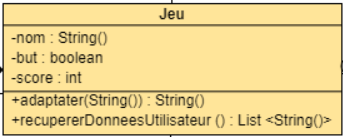
\includegraphics[scale=0.5]{include/Classe_Jeu.PNG}\newline
		\end{center}
		Attributs :
		\begin{itemize}
			\item nom : String() représente le nom du jeu ;
			\item but : boolean représente le but à atteindre, si atteint \texttt{but=True}, sinon \texttt{but=False};
			\item score : int représente le nombre de points accumulés par l’Utilisateur (avancement, points gagnés, etc…).
		\end{itemize}
		\medskip
		Opérations :
		\begin{itemize}
			\item[+] adaptation(String()) prend les informations venant du Modèle Utilisateur et renvoie l’Evénement adapté selon le contexte courant;
			\item[+] recupererDonneesUtilisateur() : String() renvoie les informations du Modèle Utilisateur.
		\end{itemize}

	\section{Classe Utilisateur}
		\begin{center}
			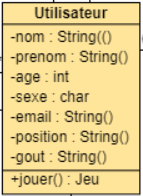
\includegraphics[scale=0.5]{include/Classe_Utilisateur.PNG}\newline
		\end{center}
		Attributs :
		\begin{itemize}
			\item nom : String() représente le nom de l’Utilisateur ;
			\item prenom : String() représente le prénom de l’Utilisateur;
			\item age : int représente l’âge de l’Utilisateur;
			\item sexe : char \texttt{F} pour Femme et \texttt{H} pour Homme;
			\item position : String() représente la position d’une personne;
			\item gout : String() représente les préférences d’une personne.
		\end{itemize}
		\medskip
		Opérations :
		\begin{itemize}
			\item[+] jouer() : Jeu est appelé lorsque l'Utilisateur fait une action dans le Jeu.
		\end{itemize}

	\section{Classe Etat Emotionnel}
		\begin{center}
			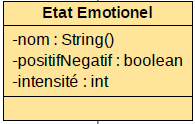
\includegraphics[scale=0.5]{include/Classe_Etat_Emotionnel.PNG}\newline
		\end{center}
		Attributs :
		\begin{itemize}
			\item nom : String() représente le nom de l’état émotionnel;
			\item positifNegatif : boolean \texttt{True} si l’état émotionnel est plutôt positif, \texttt{False} sinon;
			\item intensité : int représenté l’intensité de cet état.
		\end{itemize}

	\section{Classe Modèle Utilisateur}
		\begin{center}
			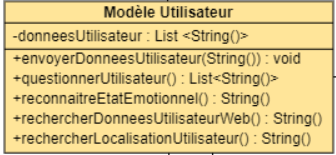
\includegraphics[scale=0.5]{include/Classe_Modele_Utilisateur.PNG}\newline
		\end{center}
		Attributs :
		\begin{itemize}
			\item donneesUtilisateur : String() représentation de l’ensemble des données
			concernant l’utilisateur sous forme de chaine de caractères
		\end{itemize}
		\medskip
		Opérations :
		\begin{itemize}
			\item[+] envoyerDonneesUtilisateur(String()) : void est l’opération permettant de transmettre les données à la classe Jeu;
			\item[+] questionnaireUtilisateur() : List<String()> retourne la liste des préférences renseignées par l'utilisateur.
			\item[+] reconnaitreEtatEmotionnel() : String() renvoie l'état émotionnel courant du joueur.
			\item[+] rechercheDonneesUtilisateurWeb() : String() renvoie une chaine de caractères contenant des données sur l'Utilisateur. Ces données ont été récupérées sur le web;
			\item[+] rechercheLocalisationUtilisateur() : String() renvoie la position courante du joueur. 
		\end{itemize}

	\section{Classe Réaction Physique}
		\begin{center}
			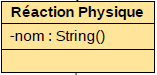
\includegraphics[scale=0.5]{include/Classe_Reaction_Physique.PNG}\newline
		\end{center}
		Attributs :
		\begin{itemize}
			\item nom : String() représente le nom de la réaction.
		\end{itemize}

	\section{Classe Réaction Physiologique}
		\begin{center}
			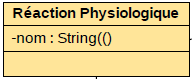
\includegraphics[scale=0.5]{include/Classe_Reaction_Physiologique.PNG}\newline
		\end{center}
		Attributs :
		\begin{itemize}
			\item nom : String() représente le nom de la réaction.
		\end{itemize}

	\section{Classe Capteur}
		\begin{center}
			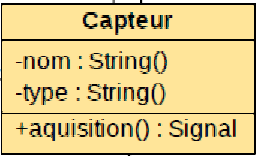
\includegraphics[scale=0.5]{include/Classe_Capteur.PNG}\newline
		\end{center}
		Attributs :
		\begin{itemize}
			\item nom : String() représente le nom du capteur;
			\item type : String() représente le type d’élément mesuré (exemple : GSR, EEG, mouvement, …).
		\end{itemize}
		\medskip
		Opération :
		\begin{itemize}
			\item[+] aquisition() : Signal permet d’enregistrer des données depuis le capteur.
		\end{itemize}

	\section{Classe Signal}
		\begin{center}
			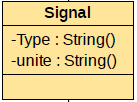
\includegraphics[scale=0.5]{include/Classe_Signal.PNG}\newline
		\end{center}
		Attributs :
		\begin{itemize}
			\item type : String() représente mesure effectuée (exemple : GSR, EEG, mouvement, …);
			\item unite : String() représente l’unité du signal.
		\end{itemize}

	\section{Classe Evénement}
		\begin{center}
			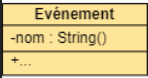
\includegraphics[scale=0.5]{include/Classe_Evenement.PNG}
		\end{center}
		Attributs :
		\begin{itemize}
			\item nom : String() représente le nom de l'événement.
		\end{itemize}

	\section{Classe Elements Externes}
		\begin{center}
			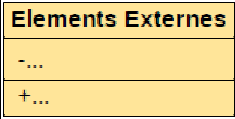
\includegraphics[scale=0.5]{include/Classe_Elements_Externes.PNG}\newline
		\end{center}
		Classe qui ne sera pas plus détaillée.
		Elle sert simplement à montrer que des éléments extérieurs au jeu sont à prendre en considération.
		C'est particulièrement vrai dans le cas du jeu pervasif.
\end{document}